\chapter{Combining Turing Machines}
\label{chap:combining}

We have defined the notion of multi-tape Turing machines and basic machines in Chapter \ref{chap:definitions}.  Now we want to construct bigger
machines, for example a single-tape machine that moves the head to the right or to a certain symbol.

\section{Control Flow Operators}
\label{sec:control}

We define control flow operators, like ``match'', ``if then else'', ``sequential composition'', and ``while''.
As a result, we get a shallow-embeded language for programming multi-tape Turing machines in an imperative way.

\subsection{Match}
\label{sec:match}

Asperti and Ricciotti \cite{asperti2015} also define the control flow operators sequential composition, conditional, and while.  However, for the
conditional they have to give one explicit ``else'' state.  Giving an explicit state is very tedious for complex machines.  That is why we use the
generalised notion of partioned machines.  For example, for the conditional $\If{M_1}{M_2}{M_3}$, $M_1$ is partitioned over $\Bool$.  If $M_1$
terminated in a ``positive'' state (i.e. a state beloning to the partition $\true$), $M_2$ is executed after $M_1$.  Else it executes $M_3$ after
$M_1$.  We observe that sequential composition and conditional can be defined as instances of a more general operator we call $\MS{Match}$.

Let $M : \TM_\Sigma^n(F)$ and $f \from F \to \TM_\Sigma^n(F')$ be a function from partitions to machines.  We define
$\MS{Match}~M~f : \TM_\Sigma^n(F')$.

\begin{definition}[$\MS{Match}~M~f$]
  \label{def:Match}
  \begin{alignat*}{3}
    & Q                  &~:=~& Q_M +  \sum_{y:F} Q_{f(y)} \\
    & start              &~:=~& \inl start_M \\
    \delta ~&(\inl q, s) &~:=~&
    \begin{cases}
      \bigl(\inr (part_M~q, start_{f (part_M~q)}), (\None, N)^n \bigr) & halt_M(q) \\
      \Let{(q', a) := \delta_M(q, s)}{\left(\inl q', a \right)} & \lnot halt_M(q)
    \end{cases} \\
    \delta ~&(\inr q, s) &~:=~& \Let{(q', a) := \delta_{f(\pi_1 q)} (\pi_2 q, s)}{\bigl( \inr (\pi_1 q, q'), a \bigr)} \\
    halt   ~&(\inl  q)   &~:=~& \false \\
    halt   ~&(\inr  q)   &~:=~& halt_{f(\pi_1~q)} (\pi_2~q) \\
    part   ~&(\inl  q)   &~:=~& \_ \\
    part   ~&(\inr  q)   &~:=~& part_{f(\pi_1~q)} (\pi_2~q)
  \end{alignat*}
\end{definition}

In Definition~\ref{def:Match}, the $part$ value for $\inl$ is unimportant, because the states of $M_1$ are not terminating states.  We just use a
canonical value.

\begin{figure}
  \center
  \documentclass{standalone}

%%%
%%% Shared preamble for all files, e.g. thesis, TikZ standalones, slides, etc.
%%% It defines \macros for types, Turing machines, etc.
%%%

% Packages needed
\usepackage[utf8]{inputenc}
\usepackage{geometry}
\usepackage[small,compact]{titlesec}
\usepackage[final]{listings}
\usepackage{amsmath}
\usepackage[amsmath,hyperref,thmmarks]{ntheorem}
% Warning: The package ntheorem defines a \None macro!
\usepackage{amssymb}
\usepackage{tipa}
\usepackage[english]{babel}
\usepackage{lstautogobble}
\usepackage{proof}
\usepackage{bussproofs}
\usepackage{xparse}
\usepackage{needspace}
\usepackage{xspace}
\usepackage{mathpartir}
\usepackage{stmaryrd} % for |llbracket and \rrbracket
\usepackage{standalone} % useful to out-source graphics


% TikZ ist *kein* Zeichenprogramm.
\usepackage{tikz}
\usetikzlibrary{arrows,shapes,snakes,automata,backgrounds,fit,positioning}
\usepackage{tikz-cd} % for commutative diagrams


%% Formating
\newcommand{\MS}[1]{\ensuremath{\mathsf{#1}}}
\newcommand{\MST}[1]{${\mathsf{#1}}$}
\newcommand{\IsMathMode}{\ifmmode{This is math mode}\else{This is not math mode}\fi}

%% Logic symbols
\newcommand{\defop}{\mathop{:=}}
\newcommand{\imp}{\mathbin{\rightarrow}~}
\newcommand{\Imp}{\mathbin{\Rightarrow}~}
\renewcommand{\iff}{\mathbin{\leftrightarrow}}


% ++ operator:
% Source: https://tex.stackexchange.com/questions/4194/how-to-typeset-haskell-operator-and-friends
\newcommand\doubleplus{+\kern-1.3ex+\kern0.8ex}
\newcommand\mdoubleplus{\ensuremath{\mathbin{+\mkern-10mu+}}}
\newcommand{\app}{\mdoubleplus}

\newcommand{\rew}{\Rightarrow}
\newcommand{\trew}{\stackrel{\textrm{T}}\Rightarrow}
\newcommand{\llrew}{\stackrel{\textrm{L}}\Rightarrow}
\newcommand{\rlrew}{\stackrel{\textrm{R}}\Rightarrow}
\newcommand{\arew}{\triangleright}
\newcommand{\conc}{\mathop{{+}\hskip-5pt{+}}}
\newcommand{\gen}{\Rightarrow}

%% Sets
% \newcommand{\lam}[2]{\lambda#1{.}\hskip.7pt#2}
\newcommand{\setOf}[1]{\bigl\{ #1 \bigr \}}
\newcommand{\setMap}[2]{\setOf{#1~\big|~#2}}
\newcommand{\depPair}[2]{\setOf{#1~{\&}~#2}}
\newcommand{\pair}[2]{\bigl( #1 , #2 \bigr)}
\newcommand{\class}[1]{\bigl[ #1 \bigr]}
\newcommand{\choice}[1]{\bigl< #1 \bigr>}
\newcommand{\explainRel}[2]{\stackrel{\text{#1}}{#2}}
\newcommand{\family}[2]{\bigl( #1 \bigr)_{#2}}
\newcommand{\from}{:}
\renewcommand{\to}{\rightarrow}

%% Types
\newcommand{\Bool}{\mathbb{B}}
\newcommand{\Fin}{\mathbb{F}}
\newcommand{\Nat}{\mathbb{N}}
\newcommand{\Prop}{\mathbb{P}}
\newcommand{\Type}{\mathbb{T}}
\newcommand{\Unit}{\MS{1}}
\newcommand{\Option}{\mathcal{O}}
\newcommand{\List}{\mathcal{L}}
\newcommand{\Rel}{\MS{Rel}}

\newcommand{\True}{\top}
\newcommand{\False}{\bot}

%% Tapes
\newcommand{\tape}[1]{[ #1 ]}
\newcommand{\tapePointer}[1]{\underset{\uparrow}{#1}}
\newcommand{\niltape}{\tape{\tapePointer{}}}
\newcommand{\midtape}[3]{\tape{#1~\tapePointer{#2}~#3}}
\newcommand{\leftof}[2]{\tape{\tapePointer{}~#1~#2}}
\newcommand{\rightof}[2]{\tape{#1~#2~\tapePointer{}}}

% \newcommand{\niltape}{\MS{niltape}}
% \newcommand{\midtape}[3]{\MS{midtape}~#1~#2~#3}
% \newcommand{\leftof}[2]{\MS{leftof}~#1~#2}
% \newcommand{\rightof}[2]{\MS{rightof}~#1~#2}

%% Turing machine types
\newcommand{\Loop}{\MS{loop}}
\newcommand{\Tape}{\MS{Tape}}
\newcommand{\Tapes}[1]{\Tape^{#1}}
\newcommand{\TM}{\MS{TM}}
\newcommand{\Move}{\MS{Move}}
\newcommand{\Act}{\MS{Act}}
\newcommand{\Conf}{\MS{Conf}}
\newcommand{\Tau}{\Gamma}

%% Relations
\newcommand{\rif}{\mathbin{\phi}}
\newcommand{\at} [2][]{#1{|}_{#2}}
\newcommand{\att}[2][]{#1{|\mkern-1.5mu|}_{#2}}
\DeclareMathOperator{\ignoreParam}{\Uparrow}
\DeclareMathOperator{\hideParam}{\Downarrow}


%% Constructors
\DeclareMathOperator{\inl}{\ensuremath{\MS{inl}}}
\DeclareMathOperator{\inr}{\ensuremath{\MS{inr}}}
\newcommand{\Some}[1]{\left\lfloor {#1} \right\rfloor}
% \None is defined sometimes
\renewcommand{\None}{\emptyset}
\newcommand{\true}{\MS{true}}
\newcommand{\false}{\MS{false}}
\newcommand{\unit}{\MS{()}}
\newcommand{\nil}{\MS{nil}}
\newcommand{\cons}{\mathbin{::}}

%% Functions
\newcommand{\map}[2]{\ensuremath{\MS{map}~#1~#2}}
\newcommand{\maptwo}[3]{\ensuremath{\MS{map}_2~#1~#2~#3}}
\newcommand{\rev}[1]{\MS{rev}~#1}

%% Vector
\newcommand{\Vector}[1]{\left[ #1 \right]}
\DeclareMathOperator{\hd}{\ensuremath{\MS{hd}}}
\DeclareMathOperator{\tl}{\ensuremath{\MS{tl}}}
\newcommand{\length}[1]{\left| #1 \right|}
\newcommand{\blength}[1]{\bigl| #1 \bigr|}


%%
%% Encding
%%
\newcommand{\contains}{\simeq}
\newcommand{\size}[1]{\length{encode(#1)}}

%% Semantics
\newcommand{\terminates}{\mathrel{\triangleright}}
\newcommand{\TerminatesIn}{\mathrel{\downarrow}}
\newcommand{\Realise}{\mathrel{\vDash}}
\newcommand{\RealiseIn}[1]{\mathrel{\vDash^{#1}}}

%%
%% Turing Machines
%%

%% Control flow operators
\newcommand{\While}{\MS{While}}
\newcommand{\Seq}{;~}
\newcommand{\Match}{\MS{Match}}
\newcommand{\If}[3]{\MS{If}~#1~\MS{Then}~#2~\MS{Else}~#3}
\newcommand{\Let}[2]{\MS{let}~#1~\MS{in}~#2}
\newcommand{\cond}[3]{\MS{if}~#1~\MS{then}~#2~\MS{else}~#3}
\newcommand{\Nop}{\MS{Nop}}
\newcommand{\Return}[2]{\MS{Return}~#1~#2}
% \newcommand{\Return}[2]{\MS{Return}_{#2}~#1}

%% Lifts
% #1 is the machine, #2 the lifting
\newcommand{\LiftTapes}[2]{\mathop{\Uparrow_{#2}} #1}
\newcommand{\LiftAlphabet}[2]{\mathop{\Uparrow_{#2}} #1}
% #1 is the machine, #2 the alphabet lifting, and #3 the tape-lifting
\newcommand{\LiftBoth}[3]{\mathop{\Uparrow_{#2;~#3}} #1}




%%%
%%% lstlisting
%%%

% Style and language to define complex multi-line definitions similar to Coq code
\lstdefinelanguage{semicoq}{
  keywords={if,then,else,true,false,match,Match,If,Then,Else,Nop,Return,Move,Reset,DoAct,WriteMove,L,R,N},
  comment=[s]{(*}{*)},
}

%% Overlap #2 over phantom #1, e.g.
%% % XX\phalign{abcdefg}{YY}XX \\
%% % XXabcdefgXX
%% gets
%% XXYY     XX
%% XXabcdefgXX
%% Idea from https://tex.stackexchange.com/questions/212710/fill-space-created-by-phantom-with-other-text
\newcommand{\phalign}[2]{\makebox[0pt][l]{\ensuremath{#2}}\phantom{#1}}

\lstdefinestyle{semicoqstyle}{
  mathescape=true,
  keywordstyle=\textsf,
  language=semicoq,
  literate={
    {=>}{{$\Rightarrow$}}2
    {>->}{{$\rightarrowtail\,$}}2
    {<->}{{$\leftrightarrow$ }}2
    {->}{{$\to$ }}3
    {~}{{$\lnot$}}1
    {/\\}{{$\land$}}2
    {\\/}{{$\lor$}}2
    {forall}{{$\forall$}}1
    {exists}{{$\exists$}}1
    {<>}{{$\not =$}}{1}
    {<=}{{$\leq$}}{1}
    {<}{{$\lt$}}{1}
    {>=}{{$\ge$}}{1}
    {>}{{$\gt$}}{1}
    {[}{{$[$}}{1}
    {|}{{$|$}}{1}
    {]}{{$]$}}{1}
    {])}{{$])$}}{2}
    {(}{{$($}}{1}
    {)}{{$)$}}{1}
    {match}{{$\MS{match}$}}5
    {if}{{$\MS{if}$}}1
    {then}{{$\phalign{\MS{else}}{{\MS{then}}}$}}3
    {else}{{$\phalign{\MS{else}}{{\MS{else}}}$}}3
    {If}{{$\MS{If}$}}2
    {Then}{{$\phalign{\MS{Else}}{{\MS{Then}}}$}}4
    {Else}{{$\phalign{\MS{Else}}{{\MS{Else}}}$}}4
  }
}

\lstdefinelanguage{pseudocode}{
  keywords={If,Then,Else,Do,While,Reset,Return,Continue,Break},
}

\lstdefinestyle{pseudocode}{
  mathescape=true,
  language=pseudocode,
  literate={
    {:=}{{$\leftarrow$}}{2}
    {<>}{{$\not =$}}{1}
    {<=}{{$\leq$}}{1}
    {<}{{$\lt$}}{1}
    {>=}{{$\ge$}}{1}
    {>}{{$\gt$}}{1}
  }
}






%%% Local Variables:
%%% mode: LaTeX
%%% TeX-master: "thesis"
%%% End:

\begin{document}
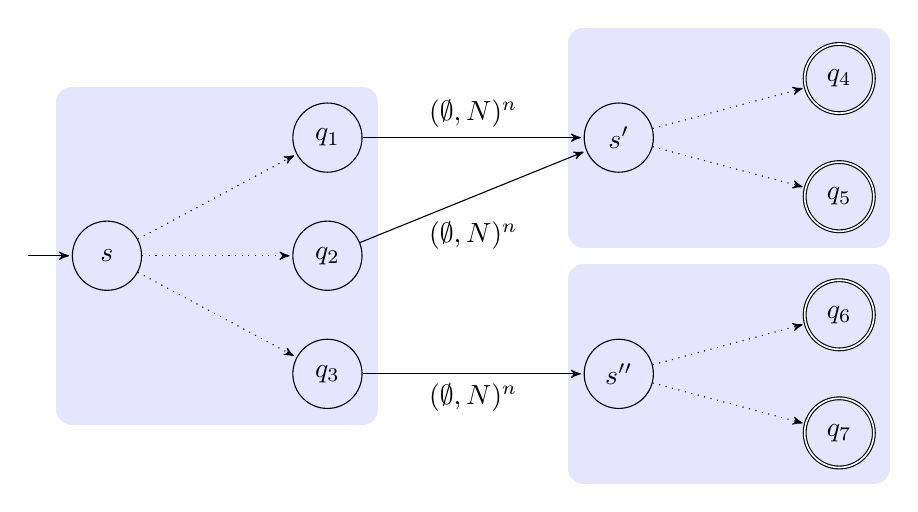
\begin{tikzpicture}[->,>=stealth',shorten >=1pt,auto,node distance=2.8cm]
  \begin{scope}
	  % Machine M
	  \node[state]          (M init)                                    {$s$};
	  \node[state]          (M exit 1)  [right of=M init,yshift= 1.5cm] {$q_1$};
	  \node[state]          (M exit 2)  [right of=M init,yshift= 0.0cm] {$q_2$};
	  \node[state]          (M exit 3)  [right of=M init,yshift=-1.5cm] {$q_3$};
	  \path (M init)
	  edge[dotted] (M exit 1)
	  edge[dotted] (M exit 2)
	  edge[dotted] (M exit 3);
	  \path (M init) ++(-1.0,0) edge (M init);
  \end{scope}
  \begin{scope}[xshift=6.5cm]
	  % Match-Machines
	  \begin{scope}[yshift=1.5cm]
		  % Accepting match machine
		  \node[state]          (M 1 init)                                        {$s'$};
		  \node[state, double]  (M 1 exit 1)  [right of=M 1 init, yshift= 0.75cm] {$q_4$};
		  \node[state, double]  (M 1 exit 2)  [right of=M 1 init, yshift=-0.75cm] {$q_5$};
		  \path (M 1 init)
		  edge[dotted] (M 1 exit 1)
		  edge[dotted] (M 1 exit 2);
	  \end{scope}
	  \begin{scope}[yshift=-1.5cm]
		  % Accepting match machine
		  \node[state]          (M 2 init)                                        {$s''$};
		  \node[state, double]  (M 2 exit 1)  [right of=M 2 init, yshift= 0.75cm] {$q_6$};
		  \node[state, double]  (M 2 exit 2)  [right of=M 2 init, yshift=-0.75cm] {$q_7$};
		  \path (M 2 init)
		  edge[dotted] (M 2 exit 1)
		  edge[dotted] (M 2 exit 2);
	  \end{scope}
  \end{scope}
  % Connecting edges
  \path
  (M exit 1) edge node[anchor=south] {$(\emptyset, N)^n$} (M 1 init)
  (M exit 2) edge node[anchor=north,yshift=-0.2cm] {$(\emptyset, N)^n$} (M 1 init)
  (M exit 3) edge node[anchor=north] {$(\emptyset, N)^n$} (M 2 init);

  \begin{pgfonlayer}{background}
	  \filldraw [line width=4mm,join=round,blue!10]
	  (M   exit 1.north -| M   init.west) rectangle (M   exit 3.south -| M   exit 3.east)
	  (M 1 exit 1.north -| M 1 init.west) rectangle (M 1 exit 2.south -| M 1 exit 2.east)
	  (M 2 exit 1.north -| M 2 init.west) rectangle (M 2 exit 2.south -| M 2 exit 2.east);
  \end{pgfonlayer}
\end{tikzpicture}

\end{document}


%%% Local Variables:
%%% TeX-master: t
%%% End:
  \caption{Example of a $\MS{Match}$.  The left box stands for the first machine $M_1:\TM_\Sigma^n(\Bool)$.  The states $q_1$ and $q_2$ are mapped to
    $\true$, $q_3$ is mapped to $\false$.  After the $\MS{Match}$ reaches one of the injections of the terminal states $q_1, \cdots, q_3$ of $M_1$, it
    continues its execution either in the top case machine $M_2$ or in the bottom case machine $M_3$.  The halting states of $\MS{Match}$ are exactly
    the injections of the halting states of the case-machines.}
  \label{fig:match}
\end{figure}

\subsubsection{Correctness of Match}
\label{sec:Match-correct}


$\MS{Match}~M~f$ first executes a copy of $M$.  When it reaches a final state $q$ of $M$, it does a ``$\MS{Nop}$'' action and changes to to the
injection of the start state of the machine $f(part~q)$.  When $\MS{Match}~M~f$ reaches a state that is the injection of a final state of a machine
$M'$, it terminates.  The correctness part of the semantics can be expressed using the following lemma:

\begin{lemma}[Correctness of $\MS{Match}~M~f$]
  \label{lem:Match_Realise}
  Let $R \subseteq \Tape_\Sigma^n \times F \times \Tape_\Sigma^n$ and $R'~y \subseteq \Tape_\Sigma^n \times F' \times \Tape_\Sigma^n$ for all $y:F$.
  If $M \vDash R$ and $f~y \vDash R'~y$ for all $y:F$, then
  \[
    \MS{Match}~M~f \vDash \bigcup_{y:F} \bigl( R\at y \circ R'~y \bigr)
  \]
\end{lemma}


\todo{Proof correctness of $\MS{Match}$}


\subsubsection{Runtime of Match}
\label{sec:match-runtime}

To specify the runtime of $\MS{Match}~M~f$, we need to know: first, the relation that $M$ realisis, second, the runtime relation in that $M$
terminates, and third, for each $y:F$ the runtime of $f~y$.


\begin{lemma}[Runtime of $\MS{Match}~M~f$]
  Let $R \subseteq \Tape_\Sigma^n \times F \times \Tape_\Sigma^n$, $T \subseteq \Tape_\Sigma^n \times \Nat$, and
  $T'~y \subseteq \Tape_\Sigma^n \times \Nat$ for all $y:F$.  If $M \vDash R$, $M \downarrow T$, and $f~y \downarrow T'~y$ for all $y:F$, then
  $\MS{Match}~M~f \downarrow \MS{MatchT}~R~T~T'$, where
  \[
    \MS{MatchT}~R~T~T' :=
    \lambda~t~i.~ \exists~i_1~i_2.~T~t~i_1 \land 1+i_1+i_2 \le i \land
      \forall~y~t'.~ R~t~y~t' \rightarrow T'~y~t'~i_2
  \]
  % (fun tin i => exists i1 i2, T1 tin i1 /\ 1 + i1 + i2 <= i /\ forall tout yout, R1 tin (yout, tout) -> T2 yout tout i2)

\end{lemma}


\subsubsection{Derived Operators}
\label{sec:match-derived-operators}

As mentioned above, conditional and sequential composition can be defined as instances of the Match operator.  For the conditional
$\If{M_1}{M_2}{M_3}$ with $M_1 : \TM_\Sigma^n(\Bool)$, $M_2, M_3 : \TM_\Sigma^n(F')$, $f$ simply maps $\true$ to $M_2$ and $\false$ to $M_3$.  For the
sequential composition $M_1 \Seq M_2$ with $M_1 : \TM_\Sigma^n(F)$ and $M_2 : \TM_\Sigma^n(F')$, $f$ maps all partitions of $F$ to $M_2$.

\begin{definition}[Conditional]
  \label{def:If}
  Let $M_1 : \TM_\Sigma^n(\Bool)$, $M_2, M_3 : \TM_\Sigma^n(F')$.
  \[
    \If{M_1}{M_2}{M_3} := \MS{Match}~M_1~
    \Bigl(
    \lambda~b.~
    \begin{cases}
      M_1 & b \\\
      M_2 & \lnot b
    \end{cases}
    \Bigr)
  \]
\end{definition}

\begin{definition}[Sequencial composition]
  Let $M_1 : \TM_\Sigma^n(F)$ and $M_2 : \TM_\Sigma^n(F')$ .
  \[
    M_1 \Seq M_2 := \MS{Match}~M_1~
    \bigl(
    \lambda~\_.~M_2
    \bigr)
  \]
\end{definition}



\subsection{While}
\label{sec:While}


The machine $\While M$ essentially behaves like a ``do-while'' loop in imperative languages like C.  At the end of the execution of the loop body $M$,
$M$ decides either to continue or break out of the loop.  If $M$ terminated in the partiton $\None$, then the loop is continued, and if $M$ terminated
in $\Some{y}$, then the loop brakes and $\While M$ terminates in $y$.  When $M : \TM_\Sigma^n(\Option(F))$, then $\While M : \TM_\Sigma^n(F)$.

$\None, \emptyset$




\section{Machine Transformations}
\label{sec:transformations}

There is a problem when we want to combine machines --- for example using sequential composition:
The number of tapes and the alphabets of both machines have to be exactly the same.
How can we re-use a single-tape Turing machine when we want to build a multi-tape machine?
How can we combine two machines with different alphabets?






\section{Examples}
\label{sec:combining-examples}




%%% Local Variables:
%%% TeX-master: "thesis"
%%% End:
